\documentclass[tikz,border=2pt]{standalone}
\usepackage{amsmath,amssymb}
\usepackage{tikz}
\usetikzlibrary{matrix}

\begin{document}
% "At most one" (y1 + y2 <= 1) forbids only the double yes; "exactly one" (y1 + y2 = 1) also
% forbids choosing nothing.
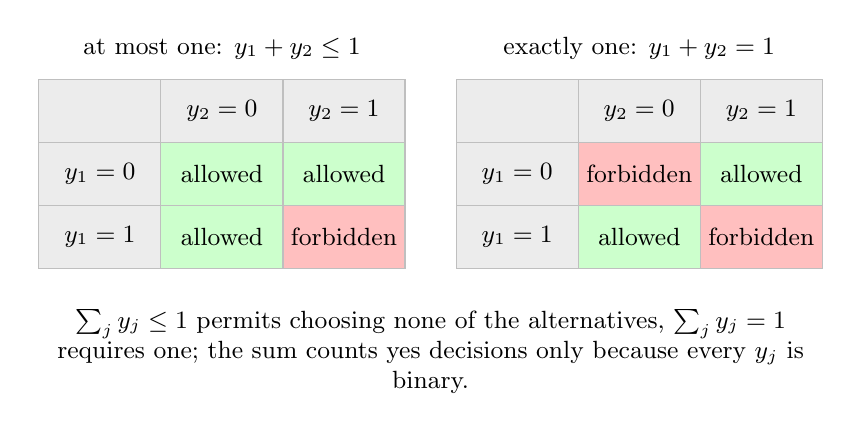
\begin{tikzpicture}[every node/.style={font=\small}]
	\matrix (A) [matrix of nodes, nodes={minimum width=1.55cm, inner xsep=2pt, minimum height=8mm, anchor=center, draw=gray!50, font=\small}, column sep=-\pgflinewidth, row sep=-\pgflinewidth] at (0,0) {
		|[fill=gray!15]| & |[fill=gray!15]| $y_2=0$ & |[fill=gray!15]| $y_2=1$ \\
		|[fill=gray!15]| $y_1=0$ & |[fill=green!20]| allowed & |[fill=green!20]| allowed \\
		|[fill=gray!15]| $y_1=1$ & |[fill=green!20]| allowed & |[fill=red!25]| forbidden \\
	};
	\node[anchor=south, font=\small] at (A.north) {at most one: $y_1+y_2\le1$};
	\matrix (B) [matrix of nodes, nodes={minimum width=1.55cm, inner xsep=2pt, minimum height=8mm, anchor=center, draw=gray!50, font=\small}, column sep=-\pgflinewidth, row sep=-\pgflinewidth] at (5.3,0) {
		|[fill=gray!15]| & |[fill=gray!15]| $y_2=0$ & |[fill=gray!15]| $y_2=1$ \\
		|[fill=gray!15]| $y_1=0$ & |[fill=red!25]| forbidden & |[fill=green!20]| allowed \\
		|[fill=gray!15]| $y_1=1$ & |[fill=green!20]| allowed & |[fill=red!25]| forbidden \\
	};
	\node[anchor=south, font=\small] at (B.north) {exactly one: $y_1+y_2=1$};
	\node[anchor=north, align=flush center, text width=10cm] at (2.65,-1.6) {$\sum_jy_j\le1$ permits choosing none of the alternatives, $\sum_jy_j=1$ requires one; the sum counts yes decisions only because every $y_j$ is binary.};
\end{tikzpicture}
\end{document}
